\begin{minipage}[t]{.6\linewidth}
  The \textbf{synthesis objective} is to \textbf{shape the norm of two filters}
  while ensuring their \textbf{complementary property}.
  This is equivalent to the conditions on the right where \(H_1(s)\) and
  \(H_2(s)\) are stable transfer function.
  $W_1(s)$ and $W_2(s)$ are \textbf{weighting functions} that are used to define
  wanted \textbf{upper bound of the complementary filter norms}.
  They should be \textbf{proper}, \textbf{stable} and \textbf{minimum phase}
  transfer functions.
\end{minipage}\hfill%
\begin{minipage}[t]{.38\linewidth}
  \vspace{-1em}
  \[ \tcmbox{\begin{align*}
       &H_1(s) + H_2(s) = 1 \\
       &|H_1(j\omega)| \le \frac{1}{|W_1(j\omega)|} \quad \forall\omega \\
       &|H_2(j\omega)| \le \frac{1}{|W_2(j\omega)|} \quad \forall\omega
     \end{align*}} \]
\end{minipage}

\bigskip

% \begin{equation*}
%   \begin{bmatrix} z_1 \\ z_2 \\ v \end{bmatrix} = P(s) \begin{bmatrix} w\\u \end{bmatrix}; \quad P(s) = \begin{bmatrix}W_1(s) & -W_1(s) \\ 0 & W_2(s) \\  1 & 0 \end{bmatrix}
% \end{equation*}

% The \(\mathcal{H}_\infty\) filter design problem is then to find a stable filter \(H_2(s)\) which based on \(v\), generates a signal \(u\) such that the \(\mathcal{H}_\infty\) norm from \(w\) to \([z_1, \ z_2]\) is less than one:
% \begin{equation*}
%   \begin{Vmatrix} \left[1 - H_2(s)\right] W_1(s) \\ H_2(s) W_2(s) \end{Vmatrix}_\infty \le 1
% \end{equation*}

% By defining \(H_1(s)\) as the complementary filter of \(H_2(s)\), we have:
% \begin{equation*}
%   \begin{Vmatrix} H_1(s) W_1(s) \\ H_2(s) W_2(s) \end{Vmatrix}_\infty \le 1
% \end{equation*}

% \begin{equation*}
%   H_1(s) \triangleq 1 - H_2(s)
% \end{equation*}

% Find $H_2(s)$ such that:
% \begin{gather*}
%   \begin{Vmatrix} \left[1 - H_2(s)\right] W_1(s) \\ H_2(s) W_2(s) \end{Vmatrix}_\infty \le 1 \\
%   H_1(s) \triangleq 1 - H_2(s)
% \end{gather*}

\bigskip

% Consider the architecture shown in Fig.~\ref{fig:h_infinity_robust_fusion} where
% $P(s)$ represents a \csquotes{generalized plant} containing the weights.

\begin{minipage}[t]{0.47\linewidth}
  This optimization problem is written as a \textbf{standard} \(\mathcal{H}_\infty\)
  \textbf{problem} (Fig.~\ref{fig:h_infinity_robust_fusion}).

  The \(\mathcal{H}_\infty\) synthesis applied to \(P(s)\) generates
  a stable filter \(H_2(s)\) such that the \(\mathcal{H}_\infty\) norm from \(w\) to \([z_1, \ z_2]\)
  is less than one.
  By defining \(H_1(s) \triangleq 1 - H_2(s)\), this is equivalent to the
  synthesis objective described above.
  \begin{tikzfigure}[$\mathcal{H}_\infty$ synthesis of
    complementary filters]
    \label{fig:h_infinity_robust_fusion}
    \centering
    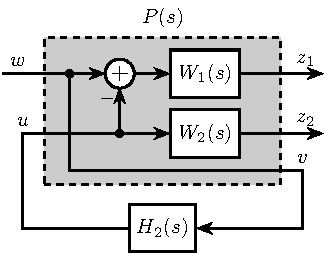
\includegraphics[scale=1.8]{figs/h_infinity_robust_fusion.pdf}
  \end{tikzfigure}
\end{minipage}\hfill
\begin{minipage}[t]{0.49\linewidth}
  This \(\mathcal{H}_\infty\) synthesis is first applied for the design of simple complementary
  filters (Fig.~\ref{fig:hinf_synthesis_results}).

  \begin{tikzfigure}[Frequency response of the weighting functions and
    complementary filters obtained using $\mathcal{H}_\infty$ synthesis]
    \label{fig:hinf_synthesis_results}
    \centering
    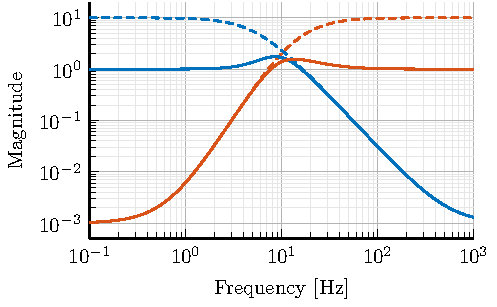
\includegraphics[width=\linewidth]{figs/hinf_synthesis_results.pdf}
  \end{tikzfigure}
\end{minipage}

% \textbf{Weighting Function Design}

% \begin{minipage}[t]{0.49\linewidth}
%   \begin{equation*}
%     W(s) = \left( \frac{
%         \hfill{} \frac{1}{\omega_0} \sqrt{\frac{1 - \left(\frac{G_0}{G_c}\right)^{\frac{2}{n}}}{1 - \left(\frac{G_c}{G_\infty}\right)^{\frac{2}{n}}}} s + \left(\frac{G_0}{G_c}\right)^{\frac{1}{n}}
%       }{
%         \left(\frac{1}{G_\infty}\right)^{\frac{1}{n}} \frac{1}{\omega_0} \sqrt{\frac{1 - \left(\frac{G_0}{G_c}\right)^{\frac{2}{n}}}{1 - \left(\frac{G_c}{G_\infty}\right)^{\frac{2}{n}}}} s + \left(\frac{1}{G_c}\right)^{\frac{1}{n}}
%       }\right)^n
%   \end{equation*}
% \end{minipage}\hfill
% \begin{minipage}[t]{0.49\linewidth}
%   \begin{tikzfigure}[Magnitude of a weighting function generated using the proposed formula \eqref{eq:weight_formula}, $G_0 = 1e^{-3}$, $G_\infty = 10$, $\omega_c = \SI{10}{Hz}$, $G_c = 2$, $n = 3$]
%     \label{fig:weight_formula}
%     \centering
%     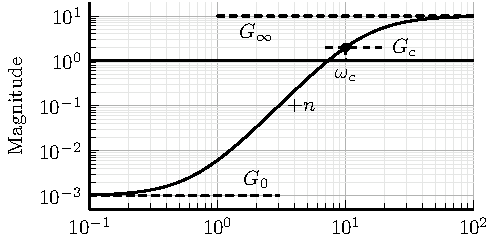
\includegraphics[width=\linewidth]{figs/weight_formula.pdf}
%   \end{tikzfigure}
% \end{minipage}

% \textbf{Three Complementary Filters}

% \begin{minipage}[t]{0.49\linewidth}
%   \begin{tikzfigure}[Architecture for $\mathcal{H}_\infty$ synthesis of three complementary filters]
%     \label{fig:comp_filter_three_hinf}
%     \centering
%     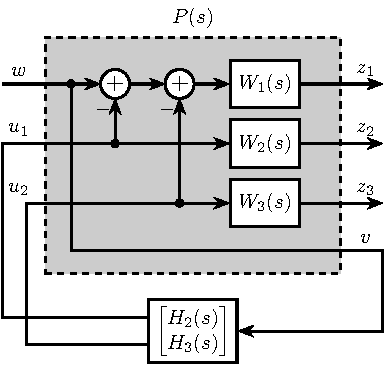
\includegraphics[scale=1.8]{figs/comp_filter_three_hinf.pdf}
%   \end{tikzfigure}
% \end{minipage}\hfill
% \begin{minipage}[t]{0.49\linewidth}
%   \begin{tikzfigure}[Frequency response of the weighting functions and three complementary filters obtained using $\mathcal{H}_\infty$ synthesis]
%     \label{fig:hinf_three_synthesis_results}
%     \centering
%     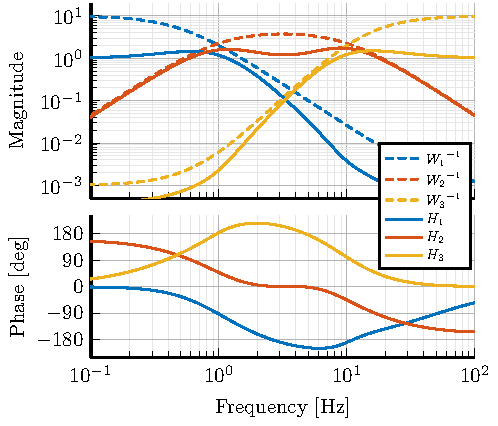
\includegraphics[scale=1.8]{figs/hinf_three_synthesis_results.pdf}
%   \end{tikzfigure}
% \end{minipage}

%%% Local Variables:
%%% TeX-master: "poster"
%%% End: